\section{Methode}
Die Bachelorarbeit wird mithilfe einer Variante des Wasserfallmodells bearbeitet werden. 
\begin{figure}[H]
  \centering
    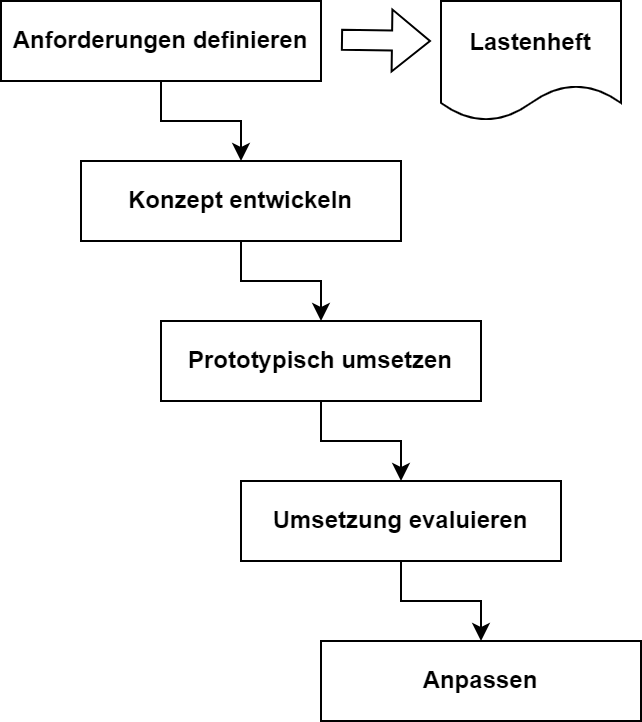
\includegraphics[width = 8cm]{bilder/wasserfallmodell}
    \caption{Wasserfallmodell Bachelorarbeit}
\end{figure}

\subsection{Anforderungen definieren}
Im ersten Schritt werden alle Anforderungen an die zu entwickelnde Software erhoben. Dabei werden sowohl geplante Features, erwünschte Ergebnisse als auch erforderliche Dokumentationen festgehalten. Anschließend wird aus den gesammelten Anforderungen ein Lastenheft erstellt.

\subsection{Konzept entwickeln}
Im zweiten Schritt des Wasserfallmodells wird das Konzept für die Software erstellt. Das Konzept besteht aus der Softwarearchitektur und dem Programmablauf. Ebenso werden hier alle verwendeten Technologien festgehalten.

\subsection{Prototypisch umsetzen}
Die anschließend erfolgende prototypische Umsetzung wird den Großteil der Bachelorarbeit ausmachen. Dort wird die Schnittstelle zwischen Datenerhebungs- und Datenverarbeitungsalgorithmen entwickelt und dokumentiert. Ebenso wird die Benutzerschnittstelle für die Einrichtung der Schnittstelle entwickelt.

\subsection{Umsetzung evaluieren}
Die Umsetzung wird nach der prototypischen Implementierung anhand des Lastenhefts evaluiert. Des Weiteren werden Probanden zur Bedienbarkeit und Verständlichkeit der Schnittstelle befragt. Dazu werden beispielhafte Daten zur Implementation vorbereitet und eine künstliche Intelligenz zur Auswertung der Daten bereitgestellt. Zur Befragung der Probanden wird ein SUS-Fragebogen verwendet. 

\subsection{Anpassen}
Zuletzt wird in der \glqq Anpassen\grqq{} Phase das Feedback der Probanden genutzt, um eventuelle Schwachstellen, Unklarheiten oder Fehler der Software zu beheben. 